\documentclass[conference]{IEEEtran}
\usepackage{graphicx} % Required for inserting images
\usepackage{cite} % For proper IEEE citation style
\usepackage{amsmath}

\title{Hype Detector: LSTM-Based Stock Price Predictions from Market Sentiment and Indicators}

\author{
    \IEEEauthorblockN{Abhinav Srivatsa, Ronith Naguri, Samiksha Racha}
    \IEEEauthorblockA{School of Computer Science and Engineering,\\
    Vellore Institute of Technology, Vellore, Tamil Nadu, India}
}

\date{October 2024} % This will be ignored in the IEEEtran class.

\begin{document}

\maketitle

\begin{abstract}
The chaotic nature of financial markets has historically posed challenges to traditional time series models like Long Short-Term Memory (LSTM), Autoregressive Integrated Moving Average (ARIMA), and Gated Recurrent Units (GRU), resulting in limited success in accurate stock price predictions. To address these limitations, this paper presents a neural network that integrates market sentiment with stock prices and technical indicators to enhance prediction accuracy. We use sentiment data from Indian financial news websites and historical stock data from Yahoo Finance. Our model combines LSTM for stock prices, dense layers for technical indicators, and an embedding layer with LSTM for sentiment analysis, providing a comprehensive approach to market forecasting. The model achieves a Root Mean Squared Error (RMSE) of 0.116 on scaled data, which corresponds to an RMSE of 1.54 INR when unscaled, against an average stock price of 244.29 INR. These results demonstrate a significant improvement over baseline models that rely solely on stock price inputs and sentiment analysis.
\end{abstract}

\section{Introduction}
Predicting stock prices has long been a central focus in financial markets, as accurate predictions can offer significant financial rewards. However, stock prices are notoriously difficult to predict due to the wide array of factors that influence market behavior, including political events, economic changes, and investor sentiment. Traditional time series models, such as Autoregressive Integrated Moving Average (ARIMA), Long Short-Term Memory (LSTM), and Gated Recurrent Units (GRU), have been widely used for stock price forecasting. While these models perform well in capturing historical trends, they often fail to account for external, non-quantitative factors like market sentiment.

The chaotic nature of the stock market, driven by a combination of technical and sentiment-related factors, has led to the exploration of new methods for prediction. Recent advances in Natural Language Processing (NLP) and Sentiment Analysis have shown that external factors like news articles and social media discussions can have a profound impact on stock prices. Integrating sentiment analysis into stock prediction models offers the potential to capture market sentiment, providing a holistic view of the market's future movements.

Despite the advancements in sentiment-based models, there remains a gap in combining market sentiment, technical indicators, and stock prices into a unified framework. This paper proposes a neural network model that integrates financial news sentiment with historical stock prices and technical indicators. Using data from Indian news websites and stock prices from Yahoo Finance, our model leverages LSTM for stock prices, dense layers for technical indicators \& sentiment scores and an embedding layer with LSTM for sentiment analysis to predict stock trends.

The contributions of this research include the integration of multiple data sources into a cohesive predictive model, yielding significant improvements in prediction accuracy. The proposed model achieves a Root Mean Squared Error (RMSE) of 1.54 INR on unscaled data, demonstrating its effectiveness in forecasting stock prices compared to baseline models that only use historical price data.

\section{Literature Review}
The early work of Bharathi and Geetha \cite{bharathi2017} used extensive preprocessing with Natural Language Processing (NLP) to analyse RSS feeds. Their predictions showcased a Multi-Layer Perceptron (MLP) to predict a rising or falling trend with a precision of 78.75\%.

Maqbool et al. \cite{maqbool2023} extended this NLP for Sentiment Analysis with an MLP and historic data to use pretrained models for sentiment scores like VADER, TextBlob, and FLAIR. They were able to predict rising and falling trends with 80\% accuracy and 100\% precision for specific stocks.

Further advancements were made by Palomo \cite{palomo}, who utilised Twitter Sentiment Analysis to predict market prices. They used FinBERT and some fine-tuned versions of it for Sentiment Analysis to achieve trend prediction with 91.3\% accuracy using a Random Forest classifier.

Q. Xiao and B. Ihnaini \cite{xiao2023} combined news and Twitter feed sentiment coupled with a "holiday effect" for additional hype analysis. They used models such as Random Forest, Naive Bayes, Logistic Regression, K-Nearest Neighbours, Support Vector Machines, and Decision Trees. The results showed a maximum accuracy of 62.4\% on a Naive Bayes model and a maximum precision of 63.5\% on a Logistic Regression model.

An approach to predictions has involved other metrics such as gold prices, fuel prices, bond yields, and USD-INR exchange rates in conjunction with Sentiment Analysis \cite{stockprice2021}. This journal paper included neural networks like Long Short-Term Memory (LSTM) and Autoregressive Integrated Moving Average (ARIMA). The regression model developed achieved a Mean Absolute Percentage Error (MAPE) of 1.6 without Sentiment Analysis and 1.25 with Sentiment Analysis.

\section{Existing Approaches}
\subsection{Sentiment Analysis with NLP and Traditional Neural Networks}
Bharathi and Geetha \cite{bharathi2017} applied extensive preprocessing with Natural Language Processing (NLP) on RSS feeds for stock prediction. Their model, based on a Multi-Layer Perceptron (MLP), was able to predict a rising or falling trend with a precision of 78.75\%. This approach laid the groundwork for integrating sentiment analysis into stock price prediction.

\subsection{Pretrained Sentiment Models with Machine Learning}
Maqbool et al. \cite{maqbool2023} extended the use of NLP for sentiment analysis by utilising pretrained models such as VADER, TextBlob, and FLAIR. Combining sentiment scores from these models with historical stock data, they achieved an 80\% accuracy and 100\% precision for predicting stock trends with an MLP model.

\subsection{Social Media Sentiment with FinBERT}
Palomo \cite{palomo} took sentiment analysis further by utilising Twitter sentiment through the use of FinBERT, a sentiment analysis model fine-tuned for financial data. Their approach, combined with a Random Forest classifier, reached an accuracy of 91.3\%, demonstrating the effectiveness of social media sentiment analysis in predicting stock prices.

\subsection{Hybrid Models Combining Multiple Machine Learning Techniques}
Q. Xiao and B. Ihnaini \cite{xiao2023} integrated news and Twitter feed sentiment with additional features like the "holiday effect" for sentiment-based stock prediction. They used a variety of machine learning models, including Random Forest, Naive Bayes, Logistic Regression, K-Nearest Neighbours, Support Vector Machines, and Decision Trees. The maximum accuracy achieved was 62.4\% using a Naive Bayes model, while the Logistic Regression model attained a maximum precision of 63.5\%.

\subsection{Incorporation of External Economic Indicators}
In addition to sentiment analysis, some approaches have incorporated external economic metrics, such as gold prices, fuel prices, bond yields, and USD-INR exchange rates, for stock price prediction \cite{stockprice2021}. Neural networks like Long Short-Term Memory (LSTM) and Autoregressive Integrated Moving Average (ARIMA) were employed, yielding a Mean Absolute Percentage Error (MAPE) of 1.6 without sentiment analysis and 1.25 with sentiment analysis.

\section{Proposed Design}
\subsection{Data Collection and Storage}
\begin{figure}
    \centering
    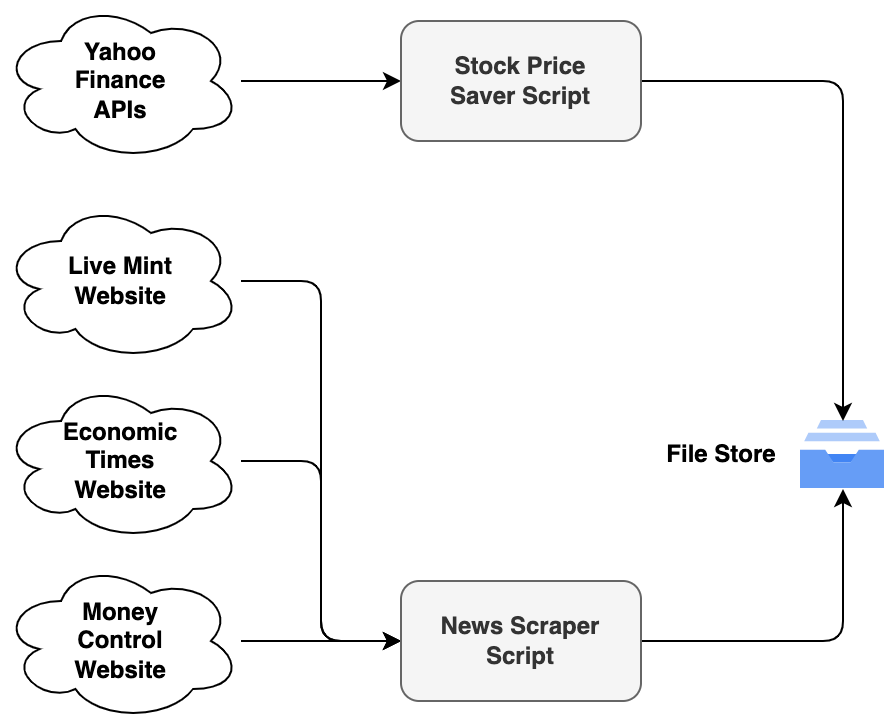
\includegraphics[width=1\linewidth]{data-collection.png}
    \caption{Flow of data collection and storage}
    \label{fig:data-collection}
\end{figure}
\subsubsection{Web Scraping for News Articles}
To collect relevant financial news, we have developed web scrapers for three major Indian financial news websites: \textit{Live Mint}, \textit{Economic Times}, and \textit{Money Control}. These scrapers extract real-time financial and market news articles, storing them for further analysis. The goal is to gather articles that may impact stock prices, such as those containing market sentiment, company news, or major economic events. All market related articles are scraped.

\subsubsection{Minute-wise Stock Data Collection}
Minute-wise stock price data is collected from \textit{Yahoo Finance}. This data includes key stock metrics such as open, close, high, and low prices, along with trading volume. Minute-wise data allows for capturing market volatility and price fluctuations on a high-frequency basis, which is essential for precise prediction models to see the real-time impact of market sentiment from news.

\subsubsection{Centralised Data Storage}
Both the financial news articles and stock price data are stored in a centralised GitHub repository. The repository ensures easy access, version control, and repeatability for future experiments. By storing both news and stock data in one location, we can maintain consistency during preprocessing and model training stages.

\subsection{Data Preprocessing}
In this section, we describe the preprocessing steps applied to both the financial news articles and the stock price data to prepare them for model training and analysis.

\begin{figure}
    \centering
    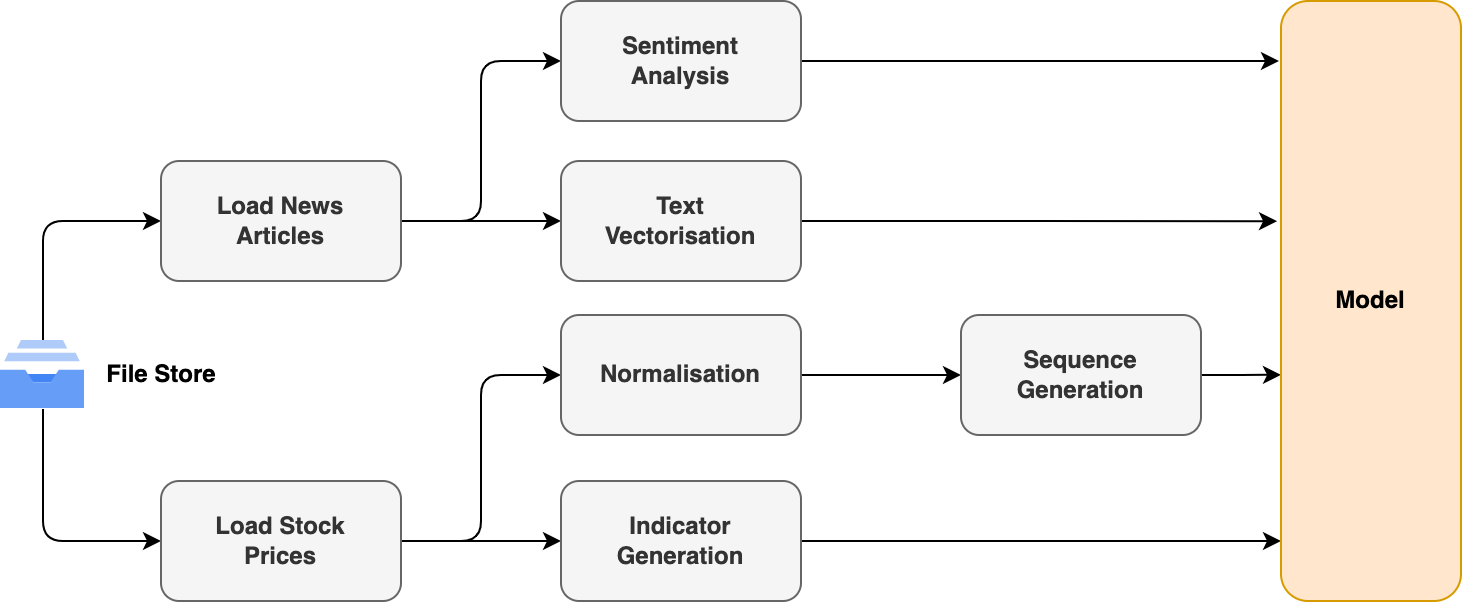
\includegraphics[width=1\linewidth]{data-preprocessing.png}
    \caption{Data preprocessing steps}
    \label{fig:data-preprocessing}
\end{figure}

\subsubsection{Generating Sequences of Stock Data}
To capture the temporal aspect of stock price movements, we first apply z-score normalization to the minute-wise close price data. This normalisation ensures that the data has a mean of 0 and a standard deviation of 1, which helps stabilize model training and prevents certain features from dominating due to scale differences.

\[
Z = \frac{X - \mu}{\sigma}
\]
\text{Where:}
\begin{itemize}
    \item \(Z\): z-score (standardised value)
    \item \(X\): original value
    \item \(\mu\): mean of the dataset
    \item \(\sigma\): standard deviation of the dataset
\end{itemize}

After normalization, we generate sequences of close price data over a fixed time window. Each sequence contains normalised close price points for a specified number of minutes, allowing us to capture short-term trends and patterns. These sequences are then used as input for time-series models.

\subsubsection{Sentiment Analysis of News Articles}
Sentiment analysis is performed on the news articles to quantify the market sentiment reflected in the text. We use the Valence Aware Dictionary and sEntiment Reasoner (VADER) sentiment analysis tool, which is specifically tuned for analysing sentiment in social media and financial contexts. VADER classifies each article as positive, negative, or neutral, assigning a sentiment score based on the intensity of the sentiment.

These sentiment scores are crucial because embedding layers in machine learning models, while effective at capturing semantic meaning, struggle to directly infer sentiment from text passages. By incorporating sentiment scores, we enhance the model’s ability to understand the emotional tone of the news, which can significantly change how a stock price moves. The sentiment scores are then integrated with the stock price data to measure the real-time effect of news sentiment on stock fluctuations.

\subsubsection{Generating Technical Indicator Features}
To enhance the predictive power of our model, we compute a range of technical indicators from the stock data. These indicators provide insights into market trends, momentum, and volatility. Below, we detail each indicator used:

\paragraph{Engulfing Candles}
An Engulfing Candle is a candlestick pattern where a larger body candle completely engulfs the body of the previous candle. A bullish engulfing pattern occurs when a small red candle is followed by a large green candle, indicating potential upward momentum and a possible trend reversal from a downtrend to an uptrend. A bearish engulfing pattern shows the opposite, signaling downward pressure and a potential reversal from an uptrend to a downtrend.
\[
\text{Engulfing} = 
\begin{cases}
\text{Bullish}, & \text{if} \text{ Close}_{i} > \text{Open}_{i} \\
& \land \text{ Close}_{i} > \text{Open}_{i-1} \\
& \land \text{ Open}_{i} < \text{Close}_{i-1} \\
\text{Bearish}, & \text{if} \text{ Close}_{i} < \text{Open}_{i} \\
& \land \text{ Close}_{i} < \text{Open}_{i-1} \\
& \land \text{ Open}_{i} > \text{Close}_{i-1} \\
\text{None}, & \text{otherwise}
\end{cases}
\]

\paragraph{Marubozo Candles}
A Marubozo Candle is a candlestick with no upper or lower shadow, meaning the stock opened and closed at its highest or lowest price for the session. A green Marubozo indicates strong buying pressure, while a red Marubozo signals strong selling pressure.
\[
\text{Marubozo} = 
\begin{cases}
\text{Bullish}, & \text{if} \text{ Close}_{i} > \text{Open}_{i} \\
& \land \text{ High}_{i} = \text{Close}_{i} \\
& \land \text{ Low}_{i} = \text{Open}_{i} \\ 
\text{Bearish}, & \text{if} \text{ Close}_{i} < \text{Open}_{i} \\
& \land \text{ High}_{i} = \text{Open}_{i} \\
& \land \text{ Low}_{i} = \text{Close}_{i} \\
\text{None}, & \text{otherwise}
\end{cases}
\]

\paragraph{Doji Candles}
A Doji Candle forms when the opening and closing prices are nearly the same, indicating indecision in the market. It often signals a potential reversal in the price trend when found at the peak or trough of price movements.
\[
\text{Doji} = 
\begin{cases}
\text{True}, & \text{if } |\text{Close}_{i} - \text{Open}_{i}| \leq \epsilon \\
& \text{where } \epsilon \text{ is a small threshold value} \\
\text{False}, & \text{otherwise}
\end{cases}
\]

\paragraph{Hammer Candles}
A Hammer Candle has a small body and a long lower shadow, indicating a possible bullish reversal after a downtrend. The long lower shadow shows that sellers pushed the price down, but buyers regained control to close near the opening price.

An Inverted Hammer looks like an upside-down hammer and signals a potential bullish reversal. The long upper shadow shows buyers attempted to push the price higher, but sellers forced it back down, which could be followed by a price increase.
\[
\text{Hammer} = 
\begin{cases}
\text{Bullish}, & \text{if} \text{ Close}_{i} > \text{Open}_{i} \\
& \land \text{ Low}_{i} < \text{Open}_{i} \\
& \land \text{ } (\text{High}_{i} - \text{Close}_{i}) \\
& \text{    } \leq k \cdot (\text{Open}_{i} - \text{Low}_{i}) \\
\text{Bearish}, & \text{if} \text{ Close}_{i} < \text{Open}_{i} \\
& \land \text{High}_{i} > \text{Open}_{i} \\
& \land \text{ } (\text{Close}_{i} - \text{Low}_{i}) \\
& \text{    } \leq k \cdot (\text{High}_{i} - \text{Open}_{i}) \\
\text{None}, & \text{otherwise}
\end{cases}
\]

\paragraph{Moving Average Convergence Divergence (MACD)}
The MACD is calculated by subtracting the 26-period Exponential Moving Average (EMA) from the 12-period EMA. The MACD line is then compared with a 9-period EMA of itself, called the signal line. When the MACD crosses above the signal line, it indicates bullish momentum, while crossing below suggests bearish momentum.
\[
\text{MACD Line} = \text{EMA}_{12} - \text{EMA}_{26}
\]
\[
\text{Signal Line} = \text{EMA}_{9}(\text{MACD Line})
\]

\paragraph{Relative Strength Index (RSI)}
The RSI is a momentum indicator that measures the speed and change of price movements. It oscillates between 0 and 100 and is used to identify overbought or oversold conditions. RSI is calculated using the following formula:
\[
RS = \frac{\text{Average Gain}}{\text{Average Loss}}
\]
\[
RSI = 100 - \frac{100}{1 + RS}
\]
An RSI above 70 suggests the stock is overbought, while below 30 indicates it is oversold.

\subsection{Neural Network Model}
In this section, we outline the architecture and components of the neural network model utilised for predicting stock price movements based on the preprocessed data. The model is designed to capture complex patterns and relationships in both the stock price data, sentiment scores derived from news articles, and keywords from the articles.




\section{Results Analysis}

\section{Conclusion and Future Work}

\begin{thebibliography}{1}
\bibitem{bharathi2017} 
S. Bharathi and A. Geetha, ``Sentiment Analysis for Effective Stock Market Prediction,'' \textit{International Journal of Intelligent Engineering and Systems}, vol. 10, no. 3, pp. 146--154, 2017, doi: 10.22266/ijies2017.0630.16.

\bibitem{maqbool2023} 
J. Maqbool, P. Aggarwal, R. Kaur, A. Mittal, and I. A. Ganaie, ``Stock Prediction by Integrating Sentiment Scores of Financial News and MLP-Regressor: A Machine Learning Approach,'' \textit{Procedia Computer Science}, vol. 218, pp. 1067--1078, 2023, doi: 10.1016/j.procs.2023.01.086.

\bibitem{palomo} 
C. Palomo and Stanford University, ``Tweet Sentiment Analysis to Predict Stock Market,'' in \textit{Stanford CS224N Custom Project}, [Thesis], Stanford University, n.d. Available: https://web.stanford.edu/class/archive/cs/cs224n/cs224n.1234/final-reports/final-report-170049613.pdf.

\bibitem{xiao2023} 
Q. Xiao and B. Ihnaini, ``Stock trend prediction using sentiment analysis,'' \textit{PeerJ Computer Science}, vol. 9, p. e1293, 2023, doi: 10.7717/peerj-cs.1293.

\bibitem{stockprice2021} 
``Stock Price Prediction using Sentiment Analysis and Deep Learning for Indian Markets,'' [Journal-article], 2021.
\end{thebibliography}

\end{document}
